\section{Analog HCAL}
Most recent update: pending\\
Contact person: Felix Sefkow (email: felix.sefkow@desy.de)
\subsection{Introduction}
With the advent of silicon photo-multipliers (SiPMs), the scintillator tile technology became a candidate for highly granular particle flow calorimetry. With analog read-out, energy and spatial resolution can be optimized independently. The particle flow performance is well understood; all published studies using PandoraPFA are based on this technology.

The CALICE AHCAL was the first large LC hadron calorimeter prototype to be exposed to test beams. Analysis is nearly complete and mostly published; the results validate the technology and the simulations.

The development of engineering solutions for a realistic detector is on its way. The integration of read-out electronics and calibration system into the detector layers has been demonstrated. The next step, an integrated stack, is being prepared. In parallel, as improved photo-sensors become available from industry, the design of the basic read-out cell -- the tile with SiPM -- is optimized with regard to mass production procedures.

\subsection{Recent Milestones; past and present R\&D}
\subsubsection{Test beam data analysis}
The following results using data taken with the first AHCAL ``physics'' prototype in 2006 -- 2011 at CERN and Fermilab have been published in peer-reviewed journals:
\begin{enumerate}
\item Detector construction, noise and aging studies~\cite{1748-0221-5-05-P05004}
\item Electromagnetic linearity and resolution~\cite{1748-0221-6-04-P04003}
\item Hadronic linearity and resolution, software compensation~\cite{1748-0221-7-09-P09017}
\item Test of particle flow algorithms (AHCAL with SiW ECAL)~\cite{1748-0221-6-07-P07005}
\item Studies using a scintillator SiPM based tail catcher~\cite{1748-0221-7-04-P04015}
\item Geant 4 validation with pion showers~\cite{1748-0221-8-07-P07005}
\item Geant 4 validation with tungsten absorber (low energy)~\cite{1748-0221-9-01-P01004}
\item Imaging capabilities, track segments~\cite{1748-0221-8-09-P09001}
\item Time structure of showers in Fe and W~\cite{1748-0221-9-07-P07022}
\item Geant 4 validation with protons~\cite{1748-0221-10-04-P04014}
\item Geant 4 validation with tungsten absorber (high energy)~\cite{Blaising:2015nla}
\end{enumerate}

We consider all of them as critical for validating a given HCAL technology. Papers~\cite{1748-0221-8-07-P07005},~\cite{1748-0221-9-01-P01004},~\cite{1748-0221-8-09-P09001},~\cite{1748-0221-9-07-P07022},~\cite{1748-0221-10-04-P04014} and~\cite{Blaising:2015nla} appeared after the ILC TDR was handed over.

\emph{Preliminary} results have been made public in the form of \emph{CALICE Analysis Notes} after thorough internal reviewing on the following topics:
\begin{enumerate}
\item Combined performance SiW ECAL + AHCAL + Tail Catcher~\cite{Calice:CAN015}
\item Leakage estimation using shower topology~\cite{Marchesini:CAN029}
\item Parameterization of pion and proton shower shapes~\cite{Calice:CAN048}
\item Analogue, Digital and Semi-Digital Energy Reconstruction~\cite{Calice:CAN049}
\item Extraction of h/e from the longitudinal shower profiles~\cite{Calice:CAN051}
\end{enumerate}

Notes~\cite{Calice:CAN048},~\cite{Calice:CAN049} and~\cite{Calice:CAN051} appeared in the time since the release of the ILC TDR. The studies are actively being followed up towards final publication; only the leakage study is presently uncovered due to lack of manpower.

Studies of the combined performance of the AHCAL in conjunction with the scintillator tungsten ECAL with MPPC readout are on-going. Results are expected later this year and will make the analysis of the first generation test beam data complete.

Data taking with a first, partially instrumented stack of the second generation has started at DESY continued in fall 2014 with electrons and hadrons at CERN. A framework for analysis software exists, but calibration and correction procedures for timing measurements still need to be developed.

The CALICE test beam results are nowadays the primary source of validation for hadron shower simulation, according to Geant 4 representatives, and extremely valuable for other HEP experiments, e.g. at the LHC, as well.

We finally note that test beam analysis plays an important role in training our students. Roughly speaking, each paper or note corresponds to one or several PhD theses. It is a distributed effort, the corresponding editors of the papers are from about 10 different groups.

\subsubsection{Optimization of the scintillator SiPM read-out cell}
\label{sec:OptimizationSiPMRO}

\begin{figure}
	\centering
	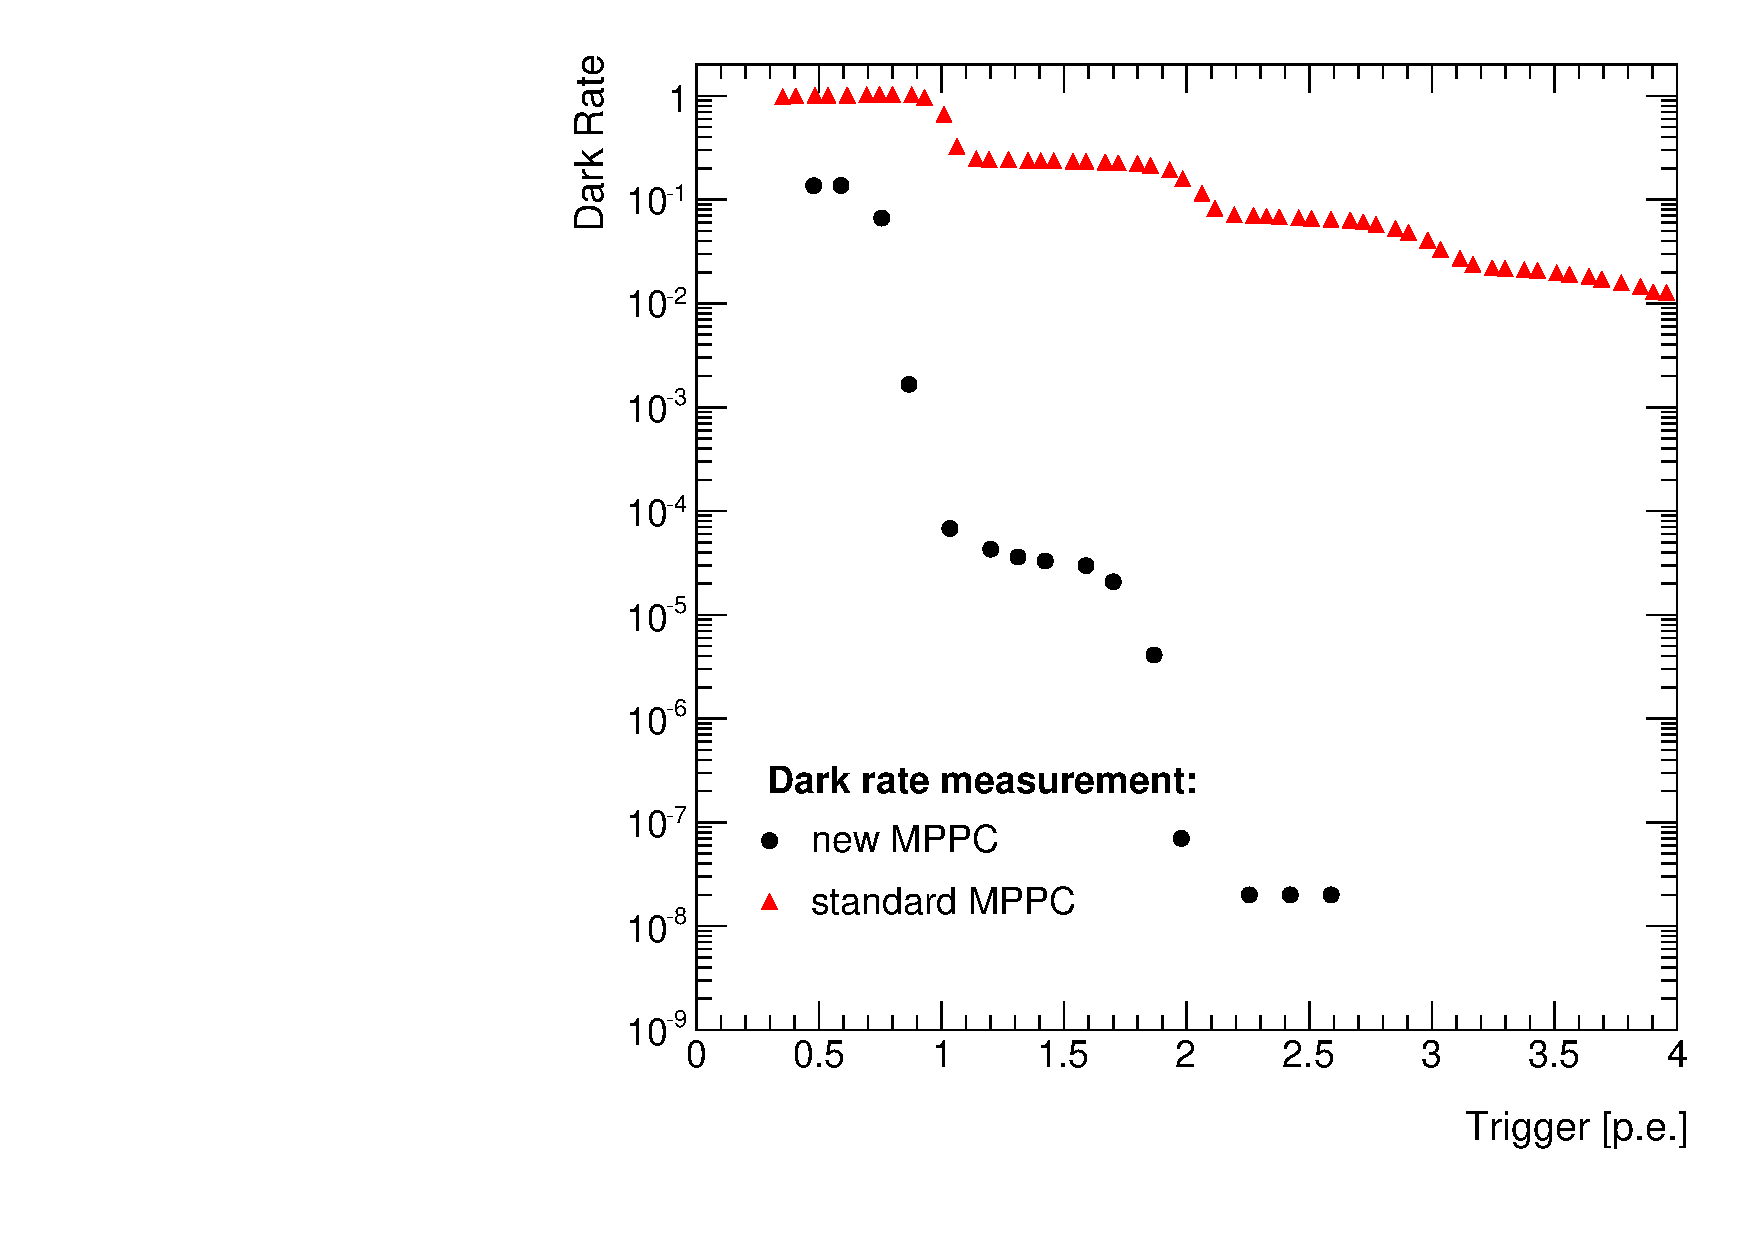
\includegraphics[width=.5\linewidth]{Calorimeter/AHCAL/DarkCount}
	\caption{Dark count rate of recent SiPMs, MPPC devices by Hamamatsu, without (standard) and with (new) inter-pixel cross talk suppression. ({\it Courtesy MPI for Physics, Munich})}
	\label{fig:Calorimeter:AHCAL:DarkCount}
\end{figure}

As a consequence of the wide success of SiPM applications in other fields, e.g. in medical imaging, the development of improved sensors is dynamically pursued in industry, and several groups are in close contact with leading producers. Progress has been made in terms of dark rate (see Figure~\ref{fig:Calorimeter:AHCAL:DarkCount}), noise above MIP threshold and dynamic range. For comparison, typical SiPMs in the first generation prototype at an the first generation had a dark rate of about 2 MHz and a cross talk probability of about 25\%. In addition, the samples are much more homogeneous than at the time of the first prototype, which results in a simplification of commissioning and calibration procedures.

In the time since the TDR, tile SiPM cells without wave-length shifting fiber have been developed. One is based on machined, individually wrapped scintillator plates, the other one on injection-molded tiles. Both are using sensors from KETEK, those on the molded tile have a very large dynamic range. 300 devices have been produced and tested, and more than thousand devices have been produced and tested with semi-automatic procedures at Hamburg and Heidelberg. They been integrated into the test beam set-up and tested at DESY and CERN in 2014 and 2015. This version is a good candidate for a baseline design for a full detector, but more data taking and analysis is needed.

Industrialisation of the SiPM and tile design and production procedures is now actively being addressed, and first assemblies with industrial facilities such as automatic pick-and-place machines have been made. This needs to be continued in the coming years, fed back into the cell optimization, and awaits a feasibility demonstration at larger scale.

\begin{figure}[htb]
	\centering
	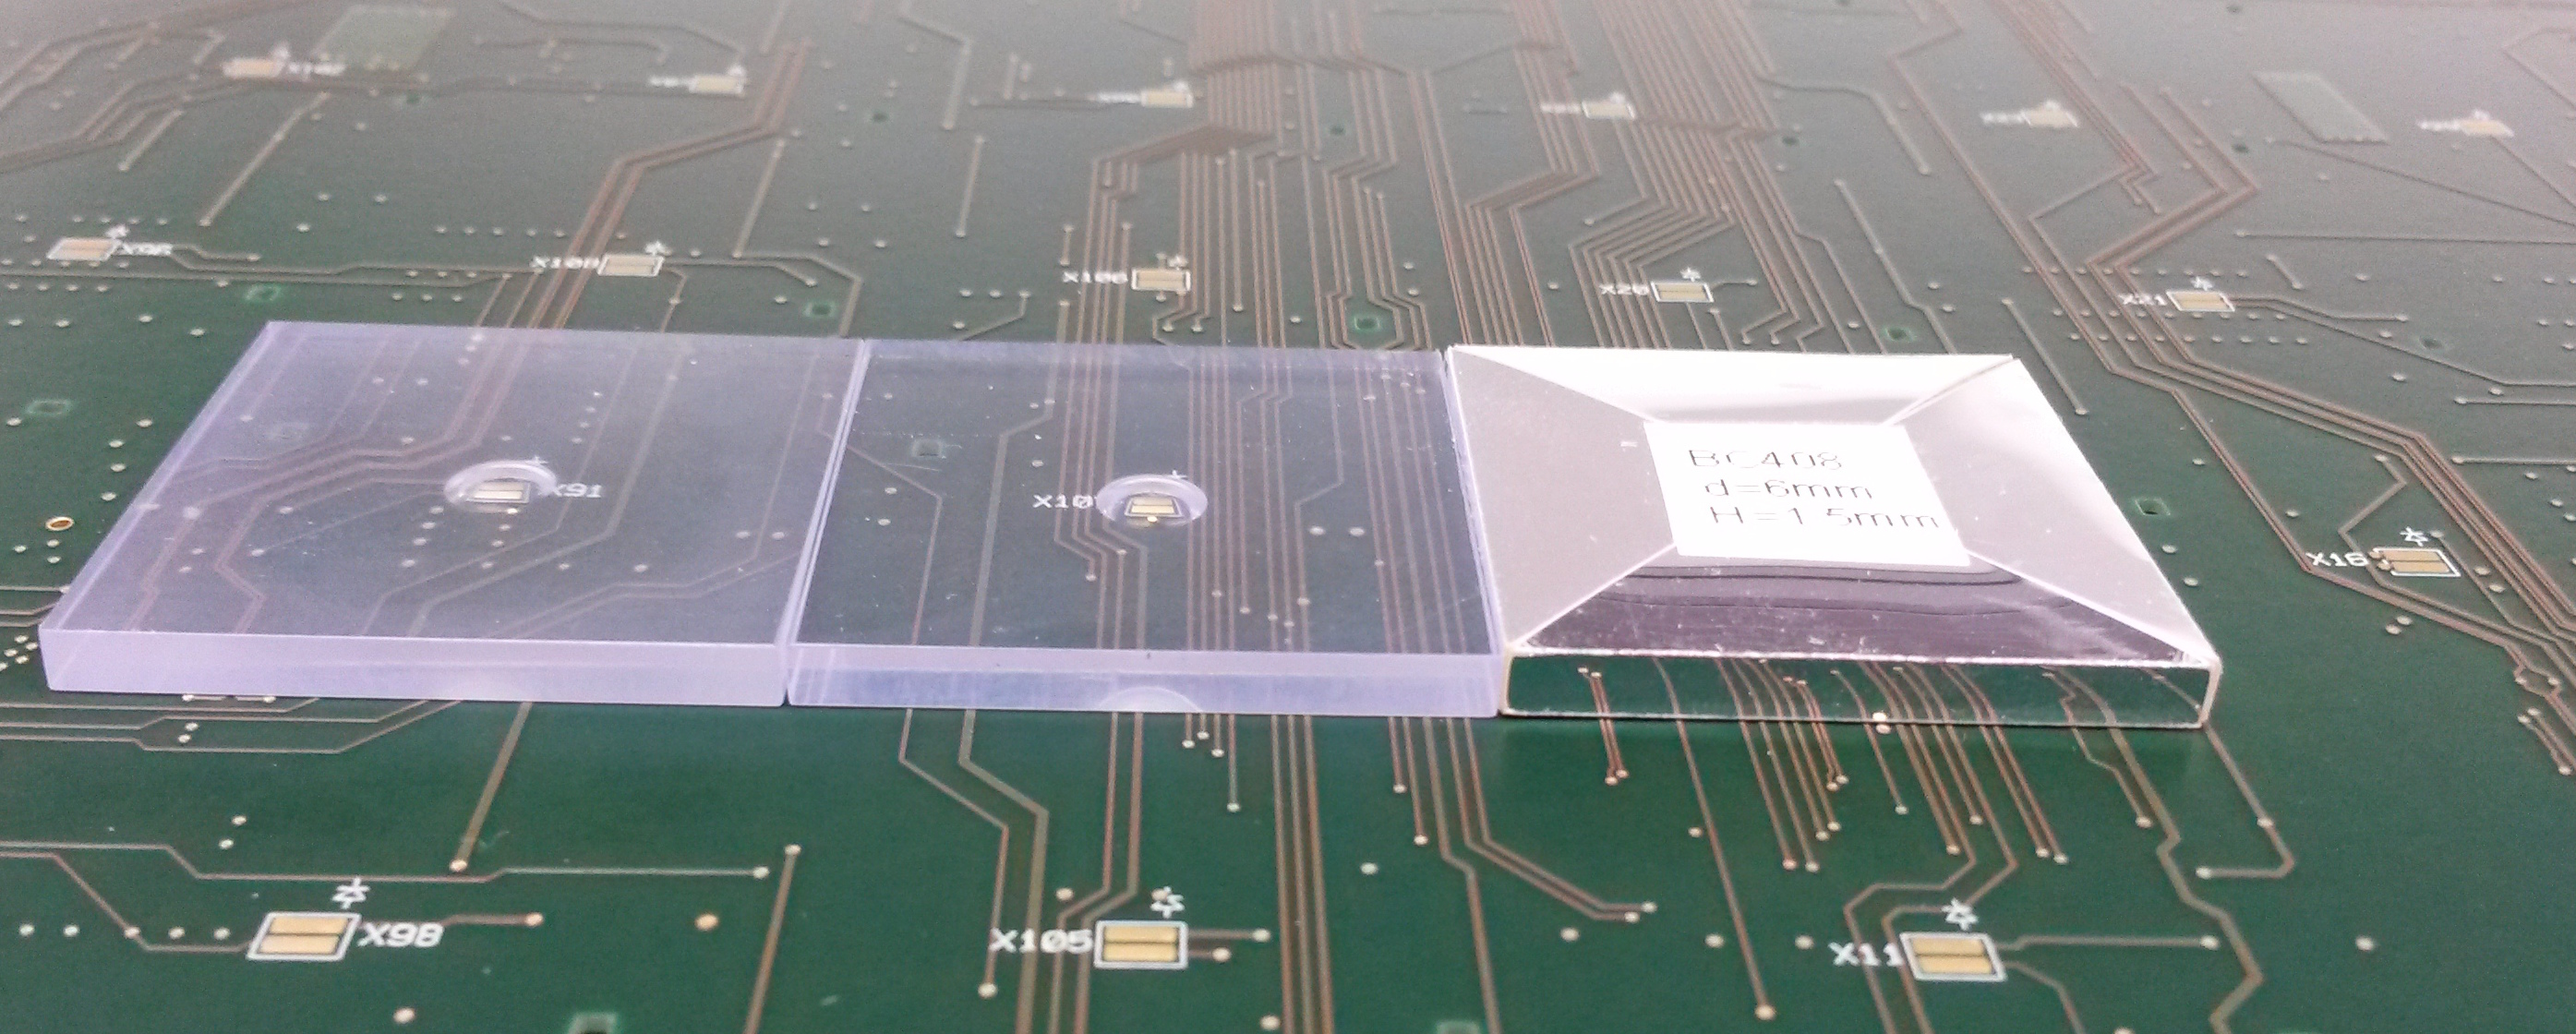
\includegraphics[width=0.5\textwidth]{Calorimeter/AHCAL/SurfaceMountedTiles}
	\caption{AHCAL read-out board with surface-mounted SiPMs and tiles. ({\it Courtesy University of Mainz})}
	\label{fig:Calorimeter:AHCAL:HBU}
\end{figure}

An alternative cell design, with photo-sensors integrated in the read-out electronics board, has been proposed some time ago, and the detailed development of the corresponding sensor and scintillator configuration is now being pursued. It has the potential to result in further simplifications (which should be read as cost and time savings), but poses higher performance requirements to the SiPM -- which can now be met --  and raises new issues in the quality assurance and integration chain. The goal is to fully develop such an alternative solution in the next 2 years. A prototype of this design is shown in Figure~\ref{fig:Calorimeter:AHCAL:HBU} and has already been successfully operated in the 2014 and 2015 test beam campaign.

\subsubsection{Electronics and active layer integration}

The design of the active layers with integrated read-out ASICs and calibration system has been basically validated in beam tests of a single HCAL layer consisting of four base units (HBUs) at CERN in 2012 and reported in the TDR. An HBU reads $12 \times 12$ tiles with 4 ASICs. The present ASIC belongs to the 2nd generation ROC family used also in ECAL and SDHCAL. An HCAL layer carries interfaces for DAQ, calibration and power supply, which already have a compact design fulfilling space constraints at an ILC detector.

The main difference between the integrated electronics and that of the physics prototype is the self-triggered operation and on-detector zero-suppression, which implies much higher demands on controlling the noise behavior and ensuring a stable detector response. It is thus mandatory to re-establish the calorimeter performance with a full-scale beam test, including the operation with fast power cycling. However, this is out of reach with present funding levels.

Further R\&D in the next years has to be done both on the ASIC and on the PCB. For the ASIC, development of a 3rd generation ROC chip will start after fixing open issues with the 2nd generation. The 3rd will have a more robust slow control architecture and possibly channel-wise buffer management which improves rate capabilities. In parallel, an alternative design of the analog part, which can handle a larger range of sensor gain needs to be complemented with a digital part.

The PCB with integrated photo-sensors, as counterpart of the corresponding tile design (see \ref{sec:OptimizationSiPMRO}), has been developed, taking automatic production and quality assurance into account. The PCB is also one of the main cost drivers of a particle flow HCAL. Dedicated R\&D, in close cooperation with industrial manufacturers, is necessary to bring the cost down. First contacts have been made, and new prototype boards have been manufactured in Korea.

\subsubsection{System integration}

\begin{figure}
	\centering
	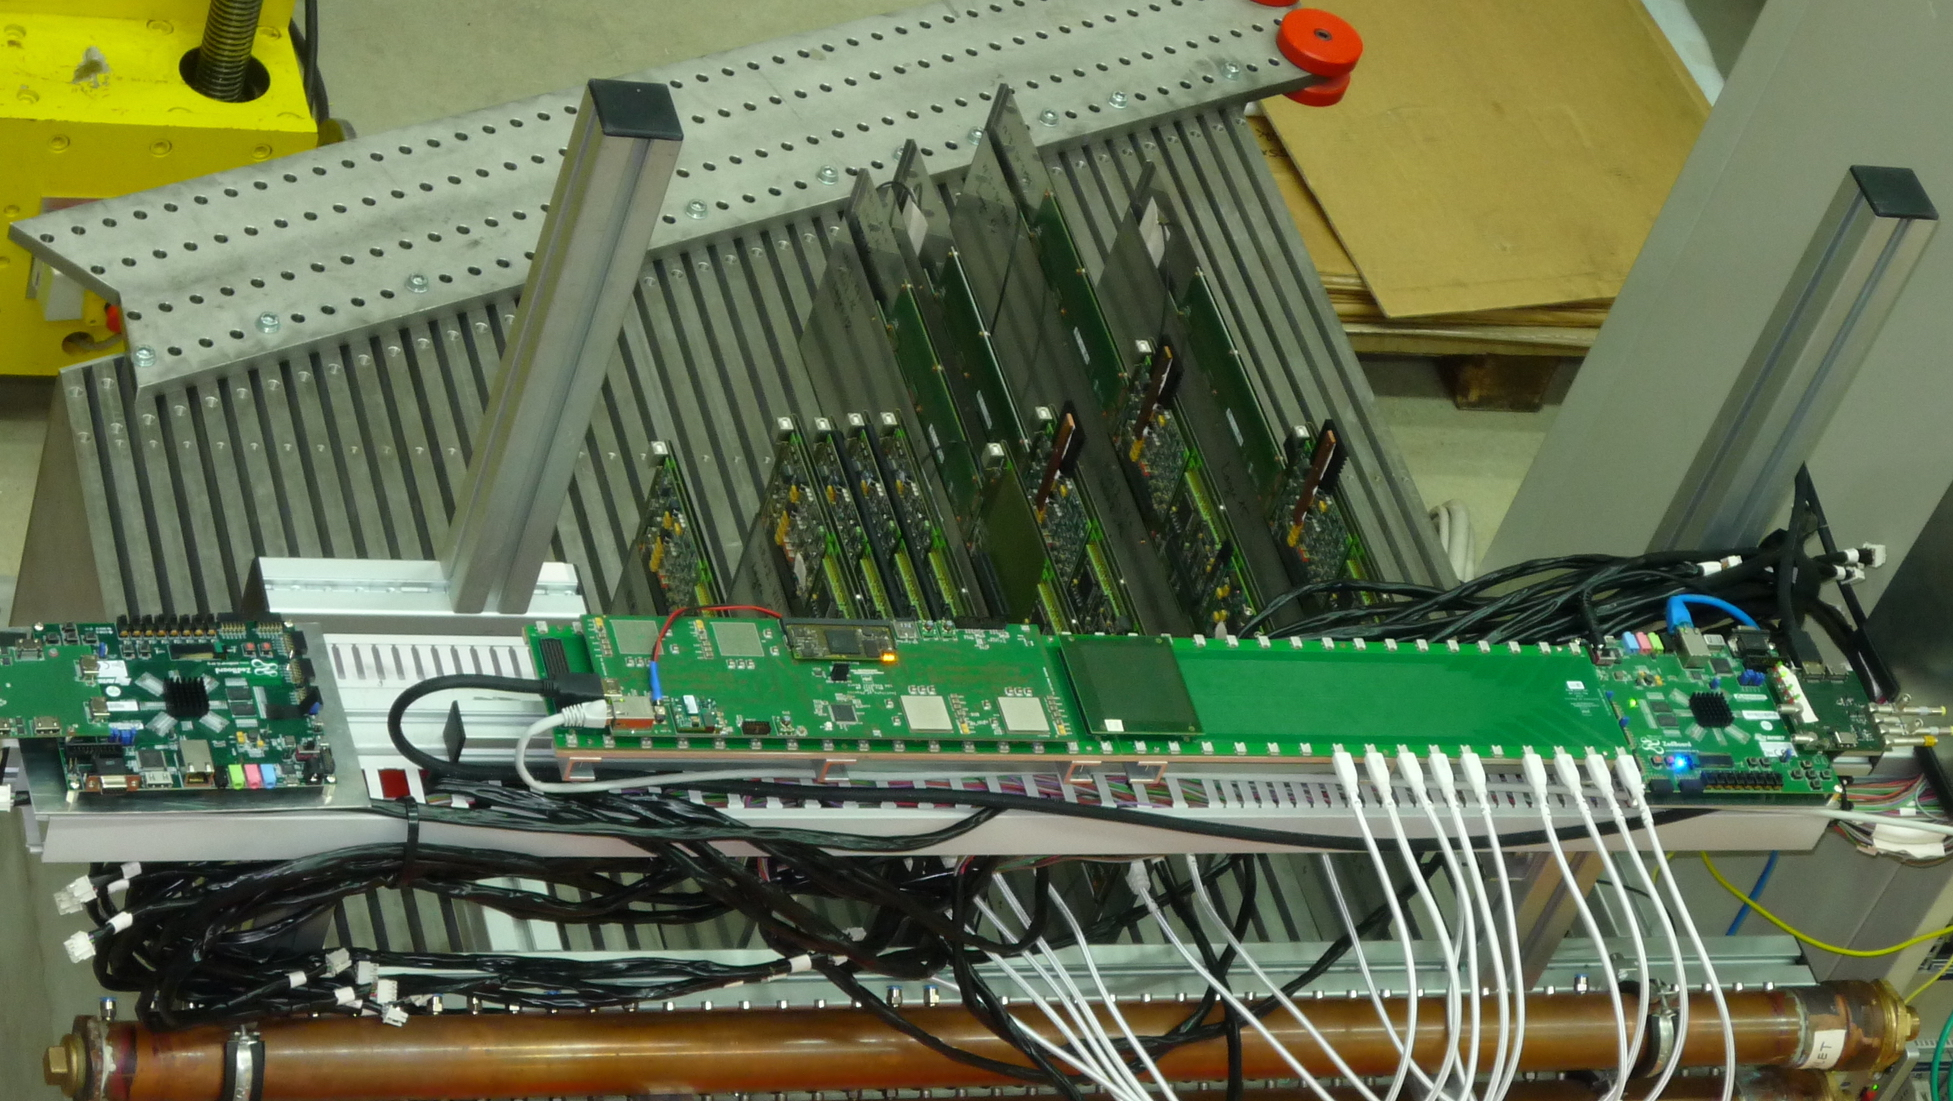
\includegraphics[width=.5\textwidth]{Calorimeter/AHCAL/AHCAL_Stack}
	\caption{AHCAL stack with integrated read-out electronics and data concentrator for two complete modules.({\it Courtesy DESY})}
	\label{fig:Calorimeter:AHCAL:Stack}
\end{figure}

While the integration of layers is well advanced, that of entire stacks or modules has only begun. Since the TDR release, efforts concentrated on developing a multi-layer DAQ capable of reading larger systems. This was ready for beam tests at CERN in fall 2014 (see Figure~\ref{fig:Calorimeter:AHCAL:Stack}). It involves integration of a dedicated module data concentrator, which collects signals from all layers for sending them to the off-detector data receiver.

Further work will be required to integrate the HCAL DAQ into a higher level system for the purpose of combined beam tests, for example with a tracking device for uniformity studies, or with an ECAL for inter-calibration and combined performance. The same is true for slow control data.

A power supply system with optimized channel density per module is being developed.

It has been demonstrated that temperature-induced variations of the SiPM gain can be compensated by adjusting the bias voltage. The approach has the potential to stabilise the detector response and trigger efficiency and thus simplify operations significantly. Automatic procedures based on this principle need to be developed and implemented for a test at system level.

On the mechanical side, a cooling system needs to be developed. The ASICs integrated in the detector layers are power-pulsed and do not need active cooling, but the interfaces, in particular the power regulators, do. A simple solution for beam tests exists, but a leak-less under-pressure based system for a large detector still needs to be prototyped.

\subsubsection{Infrastructure for production, quality assurance and characterisation}

The AHCAL is probably the sub-detector with the largest number of individual components. While the number of electronics boards, layers and interfaces is similar to other ECAL or HCAL options, the large quantity of tiles and SiPMs deserves special attention. This affects production and quality assurance, but also characterisation, i.e. test bench measurements of parameters to be used later for calibration purposes.

While it would be premature to discuss building up full production infra-structure, conceptual solutions need to be developed and exercised using demonstrators, which could be seen as prototypes of future installations. The demonstration requires reasonably large samples of detector elements, in the order of 10000, as they would be needed for a next generation full prototype.

A semi-automatic test stand for SiPMs and tiles has been developed at Heidelberg and used for the elements of the early 2014 beam test. It needs to be adapted for future designs, e.g. with SiPMs integrated in the PCB.

Automatic assembly of HBUs, i.e. of placing and soldering tiles and SiPMs on the PCB, needs to be demonstrated in practice, too. First encouraging tests with individual samples have been reported, but obviously only larger scale tests can validate the concept. A versatile cosmic test stand for the characterisation of several complete active HBUs is under development.

\subsubsection{Absorber structure}

The absorber structure bears more challenges than for conventional hadronic calorimeters. Due to the much finer longitudinal segmentation and the imperative to minimize the total radius inside the coil, there are many active gaps with tight tolerances. A design has been developed and prototyped, which achieves the required tolerances with a cost-effective roller-leveling process without machining off excess material. Two test structures have been built; one covers the full transverse cross section of a barrel module, the other the full lateral extension. The cassettes housing the active elements have the final design and are used in beam tests.

These structures need to be investigated with respect to their robustness against earthquakes. Simulations of the whole ILD structure have been made, and measurements on the test structures exposed to accelerating forces should be done in order to check the simulations.

As enough active elements become available for instrumenting several active layers at full size, the thermal simulations should be verified with measurements, too. This will constitute an important step in system integration, as it addresses the issues associated with large layers and in particular power distribution, power cycling and heat dissipation.

\subsection{Summary}
The AHCAL effort has produced a number of significant results in the time since the ILC TDR:
\begin{itemize}
\item Publication of 6 journal papers and 3 preliminary results in the form of internally reviewed notes, on Geant 4 validation with pions and protons in steel and tungsten, including new observables like track segments
\item Development, production and beam test of a new, simplified tile SiPM system without wave-length shifting fibers and improved sensor performance
\item Test with electron and hadron beams of a partially instrumented realistic absorber structure  with second generation electronics, DAQ and services
\end{itemize}

\subsection{Future Plans}

The AHCAL is ready to make the next step towards a realistic full-scale prototype and a technical design report. In order to achieve this, coordinated R\&D is required in the following areas:

Software and analysis:
\begin{itemize}
\item Completion of physics prototype test beam analysis
\item 2nd generation prototype reconstruction and simulation software
\item Development of timing reconstruction
\item Analysis of 2nd generation test beam data
\end{itemize}

Tile SiPM system:
\begin{itemize}
\item Development of scintillator SiPM system with SiPM on the PCB
\item Development of associated assembly, quality assurance and characterization procedures
\item Development of associated PCB
\end{itemize}

\subsection{Engineering Challenges}

Electronics:
\begin{itemize}
\item establish power-pulsed operation of large layers
\item 3rd generation ASIC of ROC family
\item ASIC for larger range of SiPM gains
\item PCB cost optimization
\end{itemize}

System integration:
\begin{itemize}
\item Integration of DAQ and slow control into higher level system
\item Implementation of temperature compensation scheme
\item Power supply system
\item Cooling system
\end{itemize}

Mass production concepts:
\begin{itemize}
\item Semi-automatic test stands
\item Automatic placement and soldering of tiles and SiPMs
\end{itemize}

Absorber structure:
\begin{itemize}
\item Earthquake stability calculations and tests
\item Thermal tests with full-scale instrumented and powered structures
\end{itemize}

There are ample opportunities for new groups to join into any of these fields, depending on the special competences they wish to contribute.

Particular engineering challenges are
\begin{itemize}
\item Assess and ensure earthquake stability of the absorber structure whilst maintaining a minimum of dead material
\item Developing an active layer element consisting of tiles, SiPMs and readout electronics that can be automatically assembled, including production and quality assurance procedures
\end{itemize}
